\documentclass{beamer}
\usepackage[british,spanish]{babel}
\usepackage[utf8]{inputenc}
\usepackage{hyperref}
\usepackage{multirow}



\usepackage{listings}

\usepackage{adjustbox}
\usepackage{lstcustom}

\usepackage{color}
\definecolor{light-gray}{gray}{0.80}
\definecolor{lstbackgroundshellcolor}{named}{light-gray}

\usepackage{tikz}
\newcommand*\circled[1]{\tikz[baseline=(char.base)]{
            \node[shape=circle,draw,inner sep=2pt] (char) {#1};}}

\usepackage[normalem]{ulem}

%\usepackage[acronym,xindy,toc]{glossaries}

\usepackage[acronym,xindy,toc]{glossaries}
\makeglossaries
%\usepackage[xindy]{imakeidx}
%\makeindex

\newcommand{\comment}[2]{#2}

\graphicspath{ {./images/} }

\title[Building a Scalable Architecture with Amazon SQS]{Building a Scalable Architecture with Amazon SQS}
%\subtitle[short subtitle]{long subtitle}
\author[C. Cuenca, F. Quintana]{Carmelo Cuenca-Hernández and Francisca Quintana-Domínguez}
%\institute{Escuela Universitaria de Informática}
%\date[04/2013]{Abril - 2013}
\date{}
\titlegraphic{
\includegraphics[width=0.5 \textwidth]{images/awslogo.eps}}



\pgfdeclareimage[width=2.0\baselineskip]{ulpgc-logo}{images/logosimbolo_secundario_version_vertical}
\setbeamertemplate{footline}{\raisebox{-2ex}{\pgfuseimage{ulpgc-logo}}
  \usebeamerfont{date in head/foot}\insertshortdate{}\hfill
  \usebeamertemplate{navigation symbols}\hfill
  \insertframenumber{}/\inserttotalframenumber}
\setbeamertemplate{sidebar right}{}


\usetheme{Antibes}
%\usetheme{Berlin}

%\usetheme{Warsaw}
%\usecolortheme{albatross}

\begin{document}

\begin{frame}
	\titlepage
\end{frame}


\section*{Outline}
\begin{frame}[fragile]
  \frametitle{Outline}
  %\tableofcontents%[part=1,pausesections]
  \tableofcontents[currentsection,currentsubsection, sectionstyle=show] 
  %\tableofcontents[currentsection,sectionstyle=show,hideothersubsections]
\end{frame}


\selectlanguage{british}

%%%%%%%%%%%%%%%%%%%%%%%%%%%%%%%%%%%%%%%%%%%%%%%%%%%%%%%%%%%%%%%%%%%%%%%%%%%%%%
%\newacronym{<label>}{<abbrv>}{<full>}
%\glsreset{<label>}
%\glsresetall
%\acrlong{<label>}
%\acrfull{<label>}
%\acrshort{<label>}
\newacronym{acl}{ACL}{Access Control List}
\newacronym{api}{API}{Application Programming Interface}
\newacronym{aws}{AWS}{Amazon Web Services}
\newacronym{cli}{CLI}{Command Line Interface}
\newacronym{css}{CSS}{cascading style sheets}
\newacronym{ebs}{EBS}{Elastic Block Storage}
\newacronym{ec2}{EC2}{Amazon Elastic Compute Cloud}
\newacronym{elb}{ELB}{Elastic Load Balancing}
\newacronym{iam}{IAM}{Identity Access Management}
\newacronym{ror}{RoR}{{\href{http://rubyonrails.org/}{Ruby on Rails}}}
\newacronym{rds}{RDS}{Relational Database Service}
\newacronym{rvm}{RVM}{{\href{https://rvm.io/}{Ruby Version Manager}}}
\newacronym{s3}{S3}{Simple Storage Service}
\newacronym{sqs}{SQS}{Amazon Simple Queue Service}


%%%%%%%%%%%%%%%%%%%%%%%%%%%%%%%%%%%%%%%%%%%%%%%%%%%%%%%%%%%%%%%%%%%%%%%%%%%%%
\section{Queue-Centric Workflow Pattern}
\begin{frame}[fragile,allowframebreaks]
\frametitle{Queue-Centric Workflow Pattern}
\begin{columns}
\column{0.6 \textwidth}
\begin{itemize}
\item The Queue-Centric Workflow Pattern is used in web aplications to decouple comunication between the web tier
(which implements the user interface) and the service tier (where business processing happens)
\end{itemize}
\column{0.4 \textwidth}
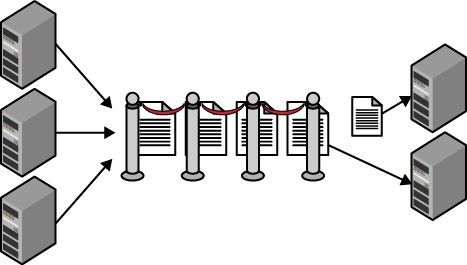
\includegraphics[width=0.75 \textwidth]{sqs.jpg}

\end{columns}
\end{frame}
%%%%%%%%%%%%%%%%%%%%%%%%%%%%%%%%%%%%%%%%%%%%%%%%%%%%%%%%%%%%%%%%%%%%%%%%%%%%%%

\section{Amazon Simple Queue Service}
\begin{frame}[fragile, allowframebreaks]
\frametitle{Amazon Simple Queue Service}
\begin{itemize}
\item \acrfull{sqs} is a fast, reliable, scalable, fully managed message queuing service. SQS makes it simple and cost-effective to decouple the components of a cloud application. You can use SQS to transmit any volume of data, at any level of throughput, without losing messages or requiring other services to be always available

\item With \acrshort{sqs}, you can offload the administrative burden of operating and scaling a highly available messaging cluster, while paying a low price for only what you use.

\item Service Highlights
\begin{itemize}
\item Reliable. Amazon \acrshort{sqs} runs within Amazon’s high-availability data centers, so queues will be available whenever applications need them. To prevent messages from being lost or becoming unavailable, all messages are stored redundantly across multiple servers and data centers
\item Scalable
\item Secure
\item Inexpensive
\end{itemize}

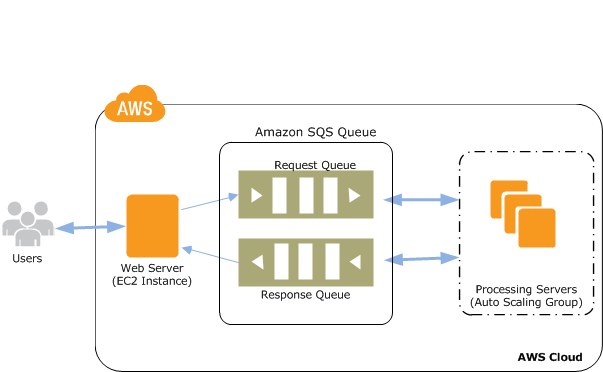
\includegraphics[width=0.75 \textwidth]{sqs-as-workflow.png}
\end{itemize}
\end{frame}
%%%%%%%%%%%%%%%%%%%%%%%%%%%%%%%%%%%%%%%%%%%%%%%%%%%%%%%%%%%%%%%%%%%%%%%%%%%%%
\begin{frame}[fragile, allowframebreaks]
\frametitle{Amazon SQS Overview}
\begin{itemize}
\item You can create any number of \acrshort{sqs} queues within the scope of your AWS account;
however, Amazon does reserve the right to delete queues if no messages have been
posted or retrieved for 30 consecutive days

\item Each queue has a name, which must be unique within a particular instance of \acrshort{sqs}
(there are currently instances of \acrshort{sqs} in the US and in Europe)
\item Every queue is identified by a unique queue URL. The URL is assigned when the
queue is created. All the operations on a queue require the specification of a queue
URL
\item Queues are used to store messages. Messages can be up to 8,192 bytes long. Due to
this low limit, messages should generally be used to pass pointers (for example,
URLs) to data stored elsewhere. Amazon \acrshort{s3} is often a good place to store data while
it’s being passed through a complex processing pipeline

\item Instead of being automatically deleted, a message retrieved from \acrshort{sqs} becomes
temporarily invisible so that it’s unable to be retrieved a second time. Once your
code retrieves a message, you have a certain amount of time—the visibility
timeout—to process and then delete the message. If the message is retained (or if
your application crashes while processing it), the message becomes visible once
again. This model allows you to build applications that avoid data loss as a result
of an application failure. The default value for the visibility timeout is 30 seconds
and the maximum value is 12 hours

\item When you retrieve a message from SQS, you also gain a receipt handle. You need
to hold on to this handle in order to delete the message after you’ve processed it.

\item Queues have a time limit: unprocessed messages will be silently deleted from the
queue after four days

\item You can choose to allow other applications and developers to access your queues
by using an access policy. The access policy gives you very granular control over
access to each aspect of SQS

\end{itemize}

\end{frame}


\section{Homework}
%%%%%%%%%%%%%%%%%%%%%%%%%%%%%%%%%%%%%%%%%%%%%%%%%%%%%%%%%%%%%%%%%%%%%%%%%%%%%
\begin{frame}[fragile]
\frametitle{Homework}
\begin{itemize}
\item ???
\end{itemize}
\end{frame}

\end{document}

\section*{Acronyms}
\begin{frame}
\frametitle[Acronyms]{Acronyms}
\glsaddall
\printglossary[type=\acronymtype] % prints just the list of acronyms
\end{frame}
%%%%%%%%%%%%%%%%%%%%%%%%%%%%%%%%%%%%%%%%%%%%%%%%%%%%%%%%%%%%%%%%%%%%%%%%%%%%%%
%%%%%%%%%%%%%%%%%%%%%%%%%%%%%%%%%%%%%%%%%%%%%%%%%%%%%%%%%%%%%%%%%%%%%%%%%%%%%%




